\documentclass[10pt,twocolumn]{article}
	
\usepackage{myfontstyle}
\usepackage{mypackages}
\usepackage{mymacros}
\usepackage{mycommands}
\usepackage{graphicx}
\usepackage{hyperref}
\usepackage{listings}
\usepackage{xcolor}


%%% This defines a style for code blocks (listings package) ----------------
\definecolor{codegreen}{rgb}{0,0.6,0}
\definecolor{codegray}{rgb}{0.5,0.5,0.5}
\definecolor{codepurple}{rgb}{0.58,0,0.82}
\definecolor{backcolour}{rgb}{0.95,0.95,0.92}

\lstdefinestyle{mystyle}{
    backgroundcolor=\color{backcolour},   
    commentstyle=\color{codegreen},
    keywordstyle=\color{magenta},
    numberstyle=\tiny\color{codegray},
    stringstyle=\color{codepurple},
    basicstyle=\ttfamily\footnotesize,
    breakatwhitespace=false,         
    breaklines=true,                 
    captionpos=b,                    
    keepspaces=true,                 
    numbers=left,                    
    numbersep=5pt,                  
    showspaces=false,                
    showstringspaces=false,
    showtabs=false,                  
    tabsize=2
}

\lstset{style=mystyle}

%%%----------------------------------------

\begin{document}
\thispagestyle{fancy1}

%%% Title and Abstract------------------------
\twocolumn[
\begin{center}
	\hrule
	\vspace{3pt}
	% Title:
	{\sffamily\bfseries\Large
		Report for Laboratory 5: Introduction to Interrupts
	} \\
	{\color{gray}
		\vspace{3pt}
		\hrule
		\vspace{3pt}
	}
	{
		\hspace*{\fill}
		Julian Soh
		\hspace*{\fill}
%		Second Author
%		\hspace*{\fill}
%		Third Author
%		\hspace*{\fill}
%		Fourth Author    % uncomment these two lines if there's a fourth author
%		\hspace*{\fill}
	}\\
	\vspace{3pt}
	{\itshape
		\hspace*{\fill}
		Department of Mechanical Engineering, Saint Martin's University
		\hspace*{\fill} \\
		\hspace*{\fill}
		ME/EE 477---Embedded Real-Time Computing for Mechanical Engineers
		\hspace*{\fill}
	}\\
	\vspace{3pt}
	{
		\hspace*{\fill}
		\today{} % today's date ... can type manually instead
		\hspace*{\fill}
	}
	\vspace{3pt}
	{\color{gray}\hrule}
%	\vspace{2pt}
\end{center}
% Abstract:
\begin{adjustwidth}{1.5in}{1.5in}
{\small
\noindent\textbf{Abstract.} \hspace{1em}
This lab explored the use of interrupts and how interrupts are handled by the FPGA of the myRIO-1900.
The interrupts will respond to an external signal, which is the trigger from an SPDT (Single Pole, Double Throw) switch.
This lab also examined the mechanical properties of the SPDT switch with respect to the electrical signals it affects and how
the use of a flip-flop to store the state of a switch will help smooth the transition and prevent noise from affecting the system. The
flip-flop circuit used in this lab was a NAND debouncing circuit.
}
\end{adjustwidth}
\vspace{9pt}
\hrule
\vspace{1\baselineskip}
]

%%% Body -------------------------

\section{Introduction} 
\label{sec:introduction}
We connected an SPDT switch to the myRIO DIO$0$ on Connector A, as shown in \autoref{fig:SPDT-myRIO}. Connector A on the myRIO
is pin 11. Other pins that were identified and used in this lab include:
\begin{itemize}
	\item DIO$0$ (pin 11)
	\item GND (pin 12)
	\item +3.3V(pin 33)
\end{itemize}

\begin{figure}[htb]
	\centering
	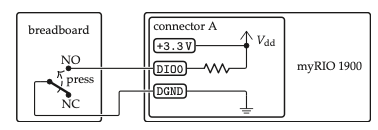
\includegraphics[width=.9\linewidth]{figures/SPDT-myRIO.png}
	\caption{Connecting SPDT directly to myRIO DIO$0$. \cite{Picone2024}.}
	\label{fig:SPDT-myRIO}
\end{figure}

The objectives of this lab were:
\begin{enumerate}
	\item To implement a system with an external interrupt
	\item To program an interrupt service routine
	\item To program multiple threads
	\item To prototype a digital logic circuit
	\item To debounce a mechanical switch
\end{enumerate}

\section{Materials and Methods}

\subsection{Materials}
The materials used in this experiment were:
\begin{itemize}
	\item Windows 10 computer with myRIO support for C and Eclipse IDE.
	\item NI myRIO-1900
	\item Rigol DHO914S Digital Oscilloscope with $25 Mhz$ function generator
	\item Rigol 712 DC power supply (to supply power to the NAND Integrated Circuit (IC)) \footnote{This was optional because we could have drawn power from the function generator of the oscilloscop or from the myRIO. But because we used this, we had to make sure the ground from this power supply is tied to the ground of the myRIO and the entire circuit so as to establish a common ground.}
	\item breadboard
	\item $1$x NAND Integrated Circuit (IC) - SN7438N
	\item $4$x 2.2 k$\Omega$ resistors
	\item Cables:
		\subitem BNC with alligator clips
		\subitem jumper cables
\end{itemize}

\subsection{Using a debouncing circuit}

After experimenting with the SPDT switch connected directly to the myRIO and observing the signal characteristics on the oscilloscope,
we implemented a debouncing circuit using a NAND gate to smooth the transitions and prevent noise from affecting the system. The schematic of
the debouncing circuit is shown in \autoref{fig:Debouncing_Circuit}.

\begin{figure}[htb]
	\centering
	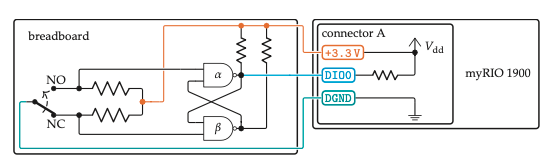
\includegraphics[width=.9\linewidth]{figures/Debouncing-circuit.png}
	\caption{Schematic of the debouncing circuit using a NAND gate. \cite{Picone2024}.}
	\label{fig:Debouncing_Circuit}
\end{figure}

The actual implementation of the debouncing circuit is shown in \autoref{fig:Debouncing_Circuit_actual}. The NAND IC was
powered by the Rigol 712 DC power supply set at +3.3V with the ground connected to the myRIO. Pin 11 of the myRIO is connected to the
output of the first NAND gate (pin 3).

\begin{figure}[htb]
	\centering
	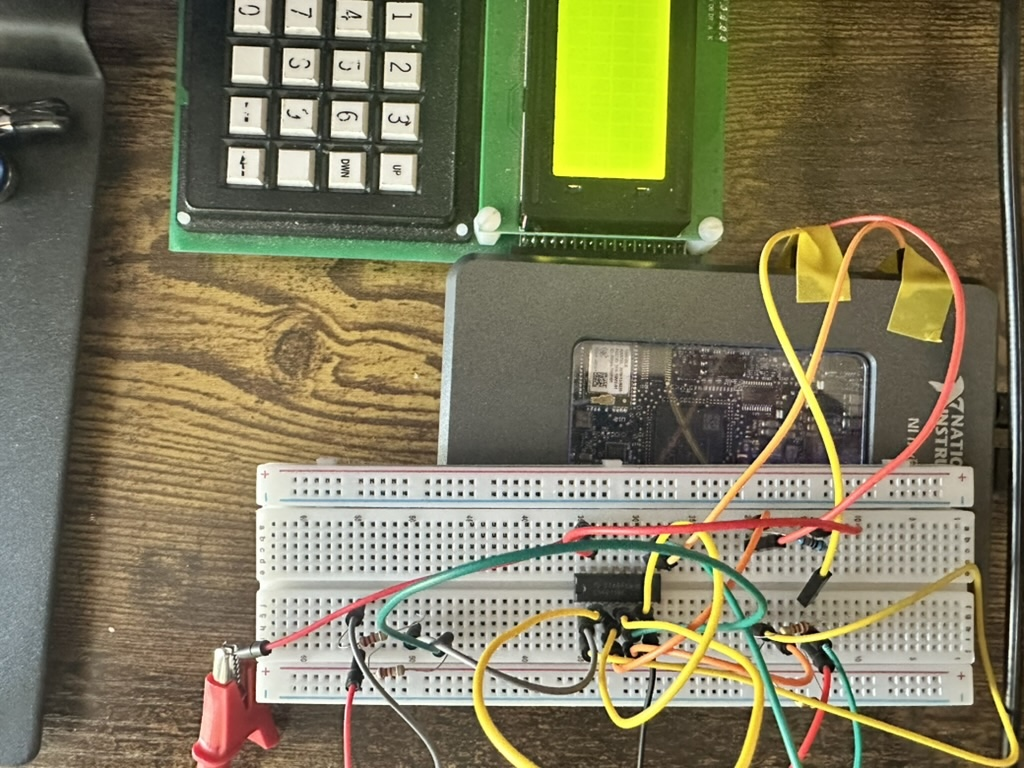
\includegraphics[width=.9\linewidth]{figures/Debouncing-circuit-actual.jpeg}
	\caption{Actual implementation of the debouncing circuit. \cite{Picone2024}.}
	\label{fig:Debouncing_Circuit_actual}
\end{figure}

\section{Laboratory Exploration and Evaluation}

The complete source code for the lab is available on GitHub at \url{https://github.com/juliansoh/ME477/blob/main/workspace/Julian_lab5/main.c}.

A video demonstration of the lab is avaiable at \url{https://github.com/juliansoh/ME477/blob/main/Reports/Lab5/videos/IMG_0052.MOV}.

\subsection{Problem L5.1}
Write and debug the \texttt{main()} and \texttt{DI\_ISR()} functions
described in section L5.2.

\vspace{\baselineskip}
See code at \url{https://github.com/juliansoh/ME477/blob/main/workspace/Julian_lab5/main.c}.



\subsection{Problem L5.2}
Provide an interrupt signal by connecting the SPDT switch on
the circuit bread board to DIO0 of connector A, as shown in figure 5.15. Notice that
pressing the switch causes a falling edge signal to be applied to the DIO0 input. Try
your program now. What happens? This undesirable phenomenon is caused by the
“bounce” of the mechanical switch. See \autoref{fig:SPDT-myRIO}.

Adjust the oscilloscope to trigger only on a high-to-low transition of the IRQ
signal. Observe several of the transitions. Typically, what length of time is required
for the transition to settle at the low level? How many triggers occur during the
settling?

\vspace{\baselineskip}
When the SPDT switched was pressed, as expected, DIO$0$ detected the signal change from high to low, thus
triggering the interrupt. The Interrupt Service Routine (ISR) was then executed. However,  we noticed that it was not a clean transition, but rather a series of rapid transitions due to the switch bouncing.
As a result, the interrupt was triggered multiple times, each triggering the ISR, resulting in printing 
"Interrupt" on the LCD numberous times as shown in \autoref{fig:SPDT-Direct-LCD1} and \autoref{fig:SPDT-Direct-LCD2}.

\begin{figure}[htb]
	\centering
	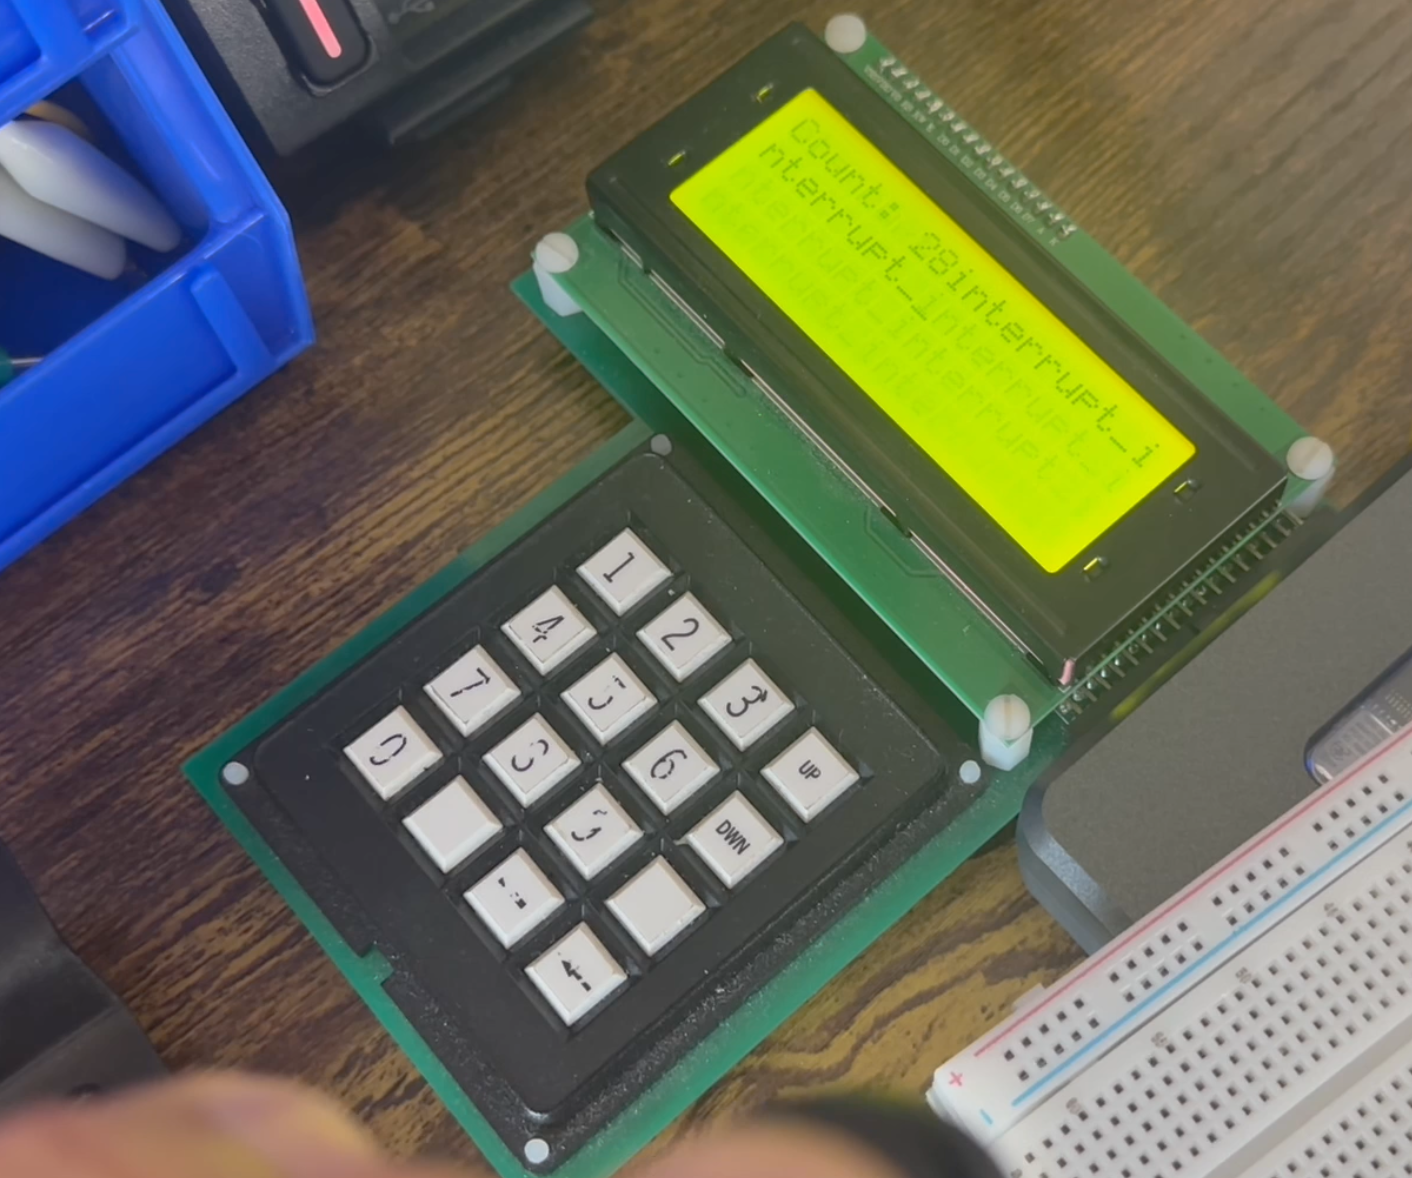
\includegraphics[width=.9\linewidth]{figures/SPDT-Direct-LCD1.png}
	\caption{LCD display showing multiple ISR execution (1 of 2).}
	\label{fig:SPDT-Direct-LCD1}
\end{figure}

\begin{figure}[htb]
	\centering
	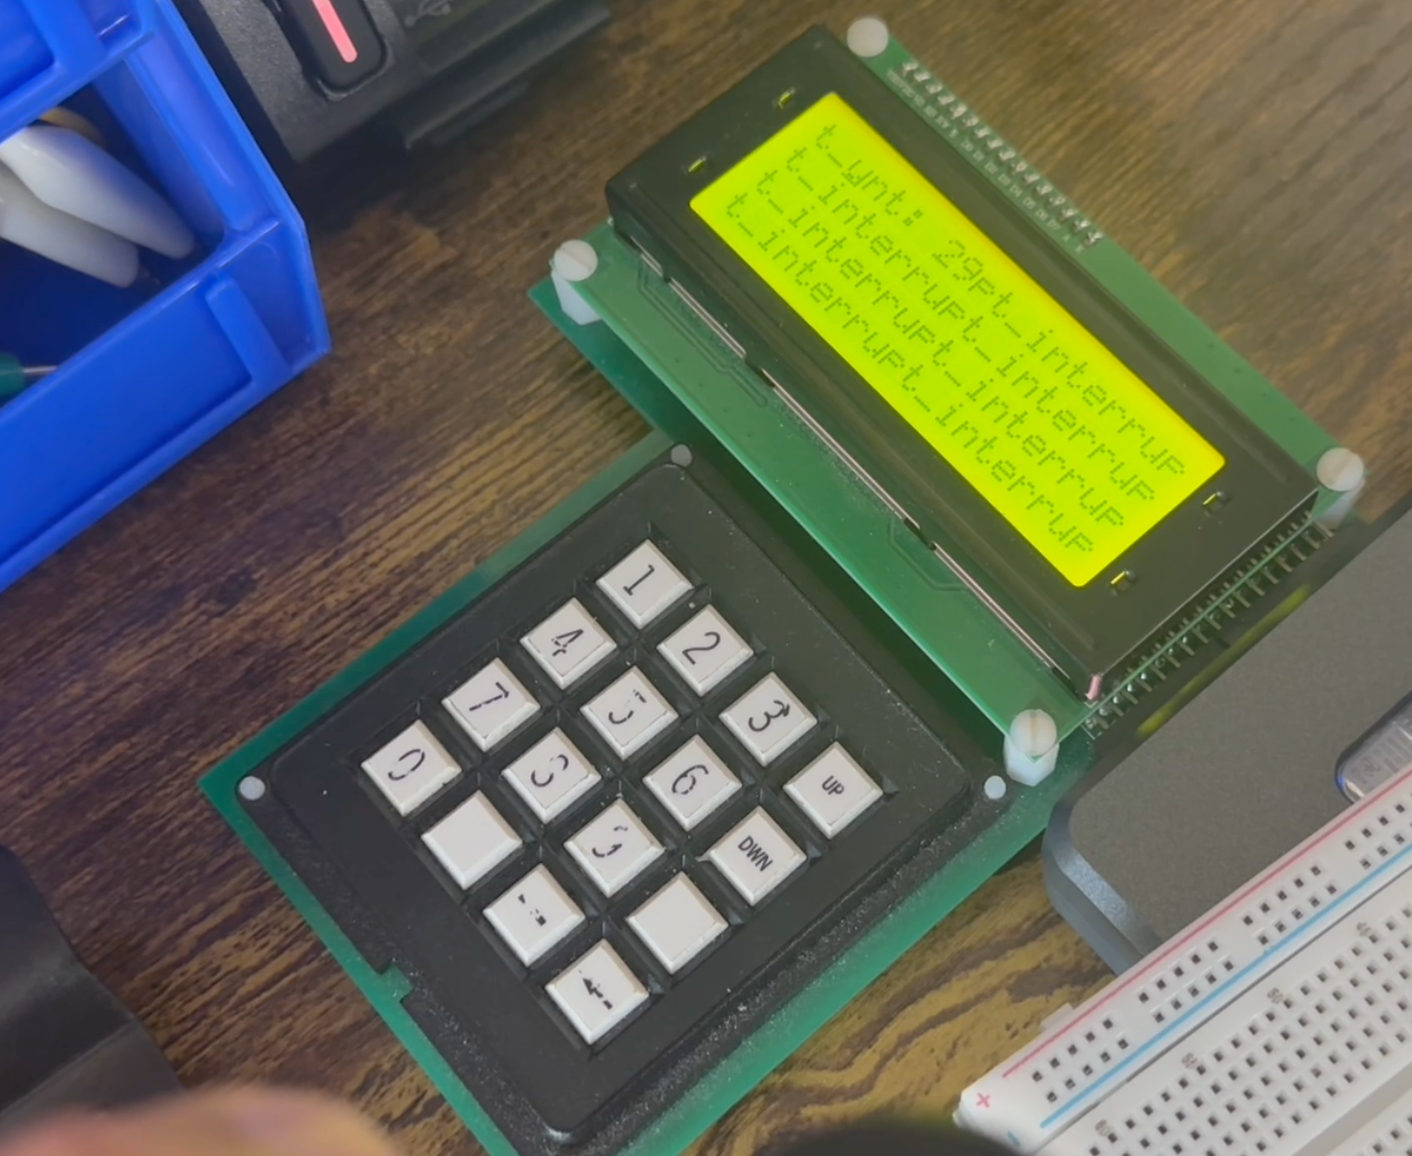
\includegraphics[width=.9\linewidth]{figures/SPDT-Direct-LCD2.png}
	\caption{LCD display showing multiple ISR execution (2 of 2).}
	\label{fig:SPDT-Direct-LCD2}
\end{figure}

Connecting the oscilloscope, we confirmed the signal went from HIGH to LOW (+$3.3V$ to $0V$) and
also observed the presence of the switch bounce based on the multiple triggers observed during the settling time, 
as shown in \autoref{fig:Rigol-SPDT-Direct1} and \autoref{fig:Rigol-SPDT-Direct2}. Therefore, instead of one press,
the myRIO interpreted the signals as multiple presses.

From what we observed, there were usually two triggers during settling, although there were a few instances
where three or more triggers occured. The multiple firing of the ISR shown in \autoref{fig:SPDT-Direct-LCD2} is
an example of when more than two triggers occured during the settling time.

\begin{figure}[htb]
	\centering
	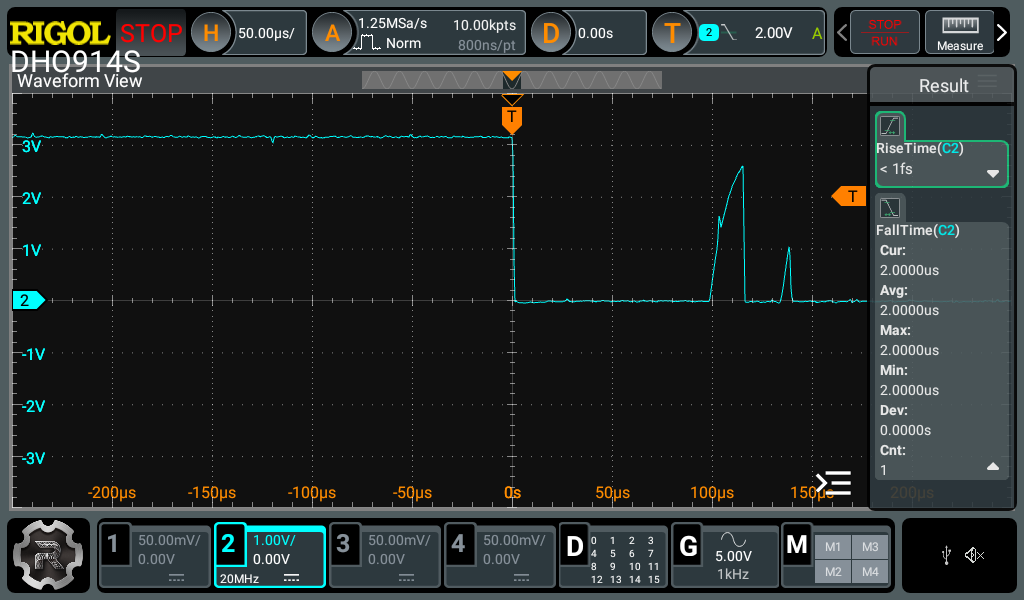
\includegraphics[width=.9\linewidth]{figures/Rigol-SPDT-Direct1.png}
	\caption{Observing switch bounce from the oscilloscope (1 of 2).}
	\label{fig:Rigol-SPDT-Direct1}
\end{figure}

\begin{figure}[htb]
	\centering
	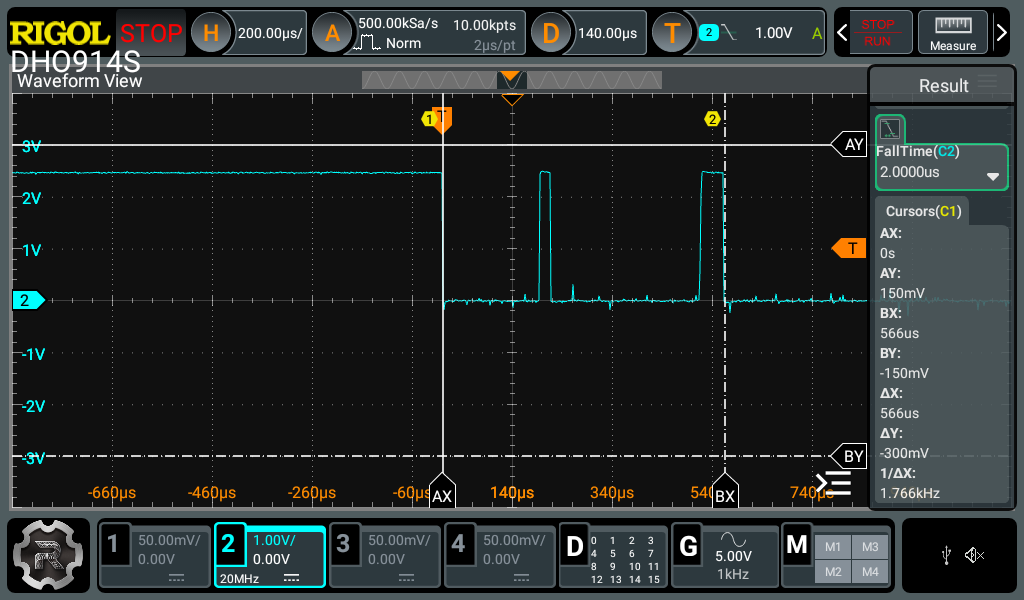
\includegraphics[width=.9\linewidth]{figures/Rigol-SPDT-Direct2.png}
	\caption{Observing switch bounce from the oscilloscope (2 of 2) WITH measurements of settling time $\Delta BX$.}
	\label{fig:Rigol-SPDT-Direct2}
\end{figure}
We used the cursor to measure the time between the initial trigger and the final stable state of the signal. As shown 
in \autoref{fig:Rigol-SPDT-Direct2}, the settling time was approximately $566 \mu s$ (See the $\boldsymbol{\Delta BX}$ reading in the right pane of the oscilloscope).
Measuring the settling time for the bounce captured in \autoref{fig:SPDT-Direct-LCD1} yielded a smaller number
of $\Delta BX = 141.5 \mu s$, as shown in \autoref{fig:Rigol-SPDT-Direct-Measure2}. Nonetheless, in both cases, we noted
that the settling times were very short and in rapid succession.

\begin{figure}[htb]
	\centering
	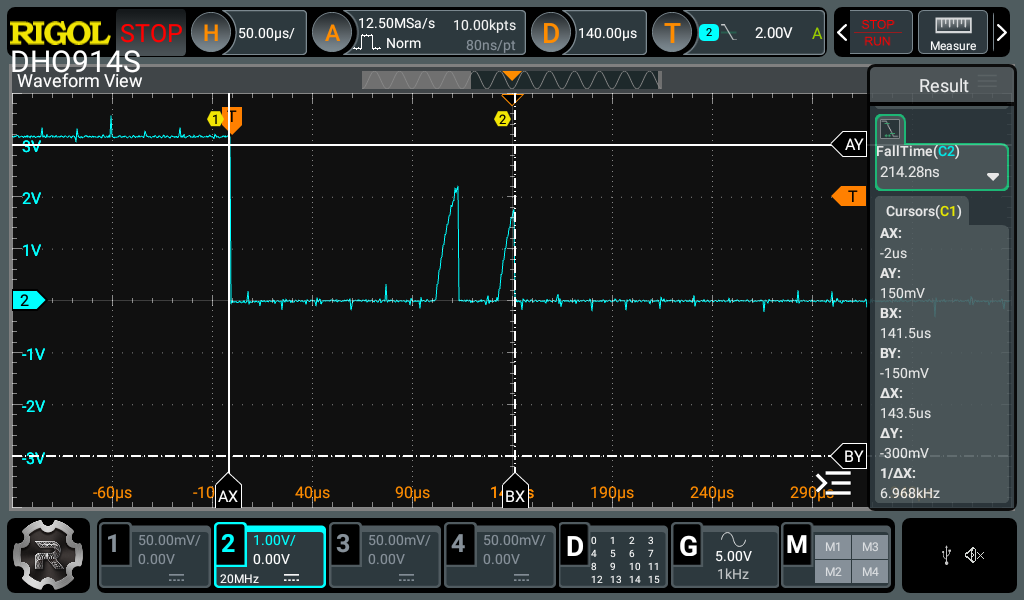
\includegraphics[width=.9\linewidth]{figures/Rigol-SPDT-Direct-Measure2.png}
	\caption{Another measurement of settling time $\Delta BX$.}
	\label{fig:Rigol-SPDT-Direct-Measure2}
\end{figure}

\subsection{Problem L5.3}
Correct the problem by replacing the switch in figure 5.15 with
the debouncing circuit shown in figure 5.16. This circuit incorporates a TTL Quad
open-collector NAND IC, (e.g., a SN7438N.)
Caution: Be certain that $V_{dd}$ and GND are connected to the chip before wiring the
rest of the circuit.
Try your program again.

\vspace{\baselineskip}
The program now only fires the interrupt once per switch press, and as such, the ISR is executed only once per switch press. The oscilloscope 
showed a clean, stable signal transition from HIGH to LOW without the multiple triggers observed previously, as can be seen in 
\autoref{fig:Rigol-NAND}.

\begin{figure}[htb]
	\centering
	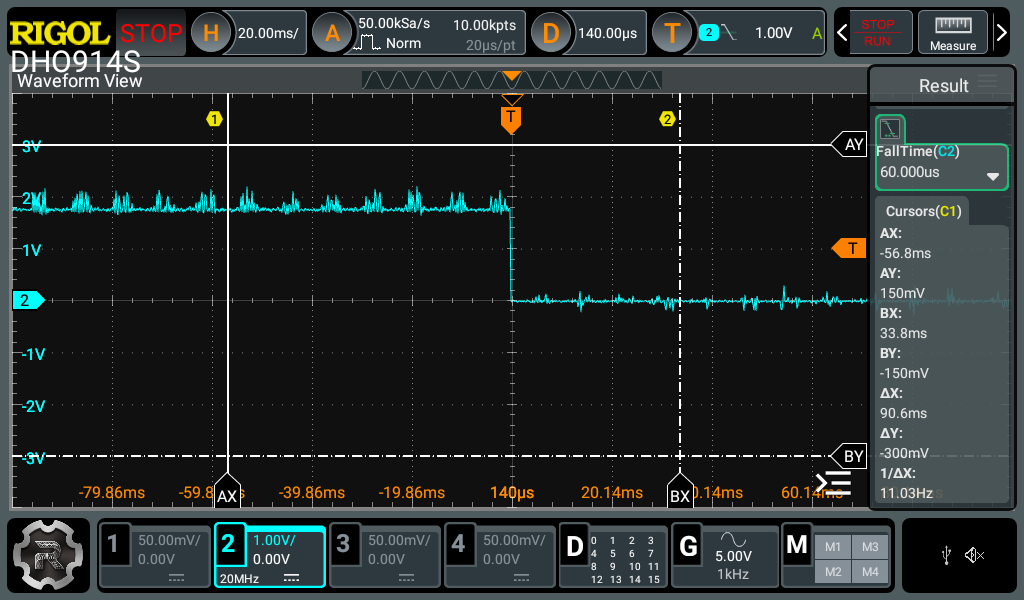
\includegraphics[width=.9\linewidth]{figures/Rigol-NAND.png}
	\caption{Oscilloscope reading of the debounced signal.}
	\label{fig:Rigol-NAND}
\end{figure}

\subsection{Problem L5.4}
Consider the switch-debouncing circuit of figure 5.13 and the
traces of the outputs/states $Q$and $Q^*$ shown in figure 5.14. Explain why each $Q$
and $Q^*$ state transition occurs and how this debounces the circuit that you built in
lab problem L5.3.

\vspace{\baselineskip}
Look at the two circuits we implemented in the lab, as portrayed by the schematic diagrams in 
\autoref{fig:Two-circuits}.

\subsubsection{Without Debouncing Circuit}

Prior to implementing the debouncing circuit, when the switch was pressed, as depicted in \autoref{fig:Two-circuits}(a), 
with $P$ connected to $DIO0$, the state of $P$ oscillated between 1 and 0 (high and low) when the switch is 
pressed because it took time to stabilize the switch and during that time, it oscillated between NO and NC. This oscillation
was captured by both the oscilloscope and the FPGA through $DIO0$.

\subsubsection{With Debouncing Circuit - Initial Conditions}
From \autoref{fig:Two-circuits}(b), this was the initial condition 
when the switch was in the "not-pressed" state.
\begin{align*}
	\overline{S} = 1 \\
	\overline{R} = 0
\end{align*}
The reason was because $V_{dd}$ flowed through the pull-up resistor then through $NO$ and to $\overline{S}$, thereby 
making $\overline{S} = 1$. The switch was closed at $NC$ so $V_{dd}$ flowed through the pull-down 
resistor to $GND$, thus $\overline{R} = 0$. Therefore, $Q^*$ will definitely be $1$ because of the NAND gate's logic.
$Q^*$ was fed back into $\alpha$, and together with $\overline{S}=1$, the output $Q$ was $0$ because of the NAND gate's logic.
\begin{align*}
	\beta: Q^* &= 1 \\
	\alpha: Q &= 0
\end{align*}

\begin{figure}[htb]
	\centering
	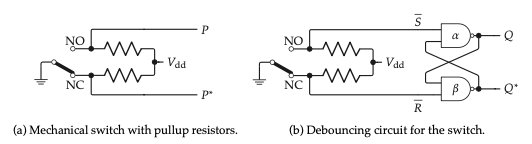
\includegraphics[width=.9\linewidth]{figures/Two-circuits.png}
	\caption{Two circuits for SPDT switch implemented in the lab. \cite{Picone2024}.}
	\label{fig:Two-circuits}
\end{figure}

\subsubsection{Switch Pressed}
When the switch was pressed, the circuit changed its state. The switch was now closed at $NO$ and open at $NC$. 
This meant that $V_{dd}$ flowed through the pull-down resistor to $GND$ and therefore made $\overline{S} = 0$.
Therefore, regardless of what the other input was for $\alpha$, $Q = 1$, which in turn fed into $\beta$.
At the same time, the switch was now closed at $NC$, so $V_{dd}$ flowed through the pull-up resistor to $\overline{R} = 1$. 
Since $Q = 1$ and $\overline{R} = 1$, the output $Q^*$ was $0$ because of the NAND gate's logic.

\begin{align*}
	\beta: Q^* &= 0 \\
	\alpha: Q &= 1
\end{align*}

\subsubsection{Switch Released}
When the switch was released, the circuit returned to its initial state.

\subsubsection{Debouncing vs Actual pressing of the switch}
The NAND IC locked in the status of Q, which was also connected to $DIO0$ that was being monitored by the FPGA on the myRIO.
The NAND flip-flop circuit ignored the noise as part of the lock-in mechanism. So even when the switch bounced, which affected Q in rapid succession,
Q did not change. The NAND IC simply ignored the noise and held the last stable state.

The question then is, how does the NAND circuit distinguish between a legitimate switch press and a bounce? Could we not
press the switch in rapid succession to simulate a bounce? For this, we look at what is definied by a legitimate
switch press. The time interval for a legitimate switch press is typically longer than the duration of a bounce, 
allowing the NAND circuit to distinguish between the two. A human pressing the swtich is ~50 to 200 ms. As we saw from 
the $\Delta BX$ measurements in \autoref{fig:Rigol-SPDT-Direct-Measure2} and in \autoref{fig:Rigol-SPDT-Direct2}, the
bounces were measured in $\mu s$. The human press is many thousands of times longer than the bounce duration. So while it is
theoretically possible to simulate a bounce via rapid succession switch presses, we conclude that in reality, this is
not physically possible, so there is no risk of encountering false negatives.

\subsection{Problem L5.5}
In your own words, explain how the main program thread
configures the interrupt thread, how it communicates with the interrupt thread
during execution, and how the interrupt thread functions.

\vspace{\baselineskip}
We defined a global data structure (ThreadResource) to hold the necessary information for the interrupt, most importantly the IRQ number (irqNumber).
We then declared an instance of ThreadResource in main() and gave the instance an arbitrary but unique irqNumber (in our case, $irqNumber = 2$).
$DIO0$ was associated to the ThreadResource instance (irqThread0) and the irqNumber and was tasked to be triggered
when a Falling Edge is detected on $DIO0$.

We then created a thread to monitor and catch $irqNumber = 2$, and when it catches this, it executes the corresponding interrupt service routine named
\texttt{DI\_ISR}. The code on what to do when the interrupt is received is defined in the \texttt{DI\_ISR} function.

\section{Author Contributions}

There is only one author for this report and lab.



%%% References -------------------------

\bibliographystyle{plainnat}
\bibliography{report}

%%% Appendices -------------------------

\end{document}  